\Grade{高一}
%\Name{1v2}\FirstTime{20181028}\CurrentTime{20181117}
\Name{林叶}\FirstTime{20180908}\CurrentTime{20181125}
% \Name{郭文镔}\FirstTime{20181111}\CurrentTime{20181117}
% \Name{马灿威}\FirstTime{20181111}\CurrentTime{20181111}
\Topic{任意角、弧度制与三角函数}
\Teach{任意角的三角函数}
\makefront
\vspace{-1.5em}
\startexercise
\hspace{-2.5em}
{\hei 本章节学习内容}\par
1. 建立一般三角函数的概念,并研究函数性质,包括周期性、奇偶性、单调性与最值;\par
2. 探索和研究三角函数之间的一些恒等关系;\par
3. 利用三角函数构建数学模型,解决实际问题。\par

\section{任意角与弧度制}
\subsection{预备知识}
1. 角与角度的概念;集合的表示;不等式的基本性质;集合的运算;直线的倾斜角;\par
2. 角度制;圆心角的性质;比例、分数的性质;圆的周长与面积;弦长的计算;锐角三角函数;二次函数最值/基本不等式.\par
\subsection{问题导学}
{\heiti 【思考1】}:角的概念是怎么产生的?我们生活中在什么时候用到过角的概念?\par
\vspace{6em}
{\heiti 【思考2】}:我们学过的角的定义是?能说出为什么这样定义么?这样定义的角可以应用在哪里呢?\par
\vspace{10em}
{\heiti 【思考3】}:为什么要定义角度?我们学过的角度是如何定义的?角度如何运算?\par
\vspace{10em}
\subsection{知识介绍}
生活中有许多“角”的形象,比如墙角的形状,斜坡,跷跷板,道路的转向,等等。把这些图像的共性抽象出来,就形成了角的最直观形象:\par
{\bf 角的静态定义}:具有公共端点的两条射线组成的图形叫做角。这个公共端点叫做角的顶点,这两条射线叫做角的两条边.\\
\begin{figure}[!htbp]
  \centering
  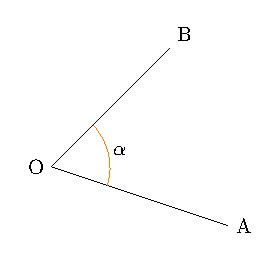
\includegraphics[scale=0.8]{Fig.ArbitraryAngle.pdf}
\end{figure}\par
{\bf 角的符号表示}:上图所示的角可记为“角AOB”、“$\angle{AOB}$”或“$\angle O$”、“角$\alpha$”或“$\angle\alpha$”
“$\alpha$”.\\
三个特殊角:{\bf\kaishu 零角,平角,直角}\par
\begin{exercise}{习题}
\item
下列说法正确的是\xz
\xx{终边相同的角一定相等}
{钝角一定是第二象限角}
{第一象限角一定不是负角}
{小于90\textdegree 的角都是锐角}
\begin{answer}B\end{answer}
\end{exercise}

\section{任意角的三角函数}
\subsection{预备知识}
1. 锐角三角函数;函数定义域
2. 勾股定理;开方;代数式化简,完全平方公式;一元二次方程求解
\subsection{问题导学}
{\heiti 【思考1】}:锐角三角函数的定义是?为什么要定义三角函数呢?三角函数有哪些应用?\par
\vspace{12em}
{\heiti 【思考2】}:锐角三角函数之间有什么关系呢?\par
\vspace{12em}

% \section{课后作业}


\stoptexercise
